% Este trabalho está licenciado sob a Licença Atribuição-CompartilhaIgual 4.0 Internacional Creative Commons. Para visualizar uma cópia desta licença, visite http://creativecommons.org/licenses/by-sa/4.0/deed.pt_BR ou mande uma carta para Creative Commons, PO Box 1866, Mountain View, CA 94042, USA.

\chapter{Arquivos e Gráficos}\label{cap_ag}
\thispagestyle{fancy}

\section{Arquivos}\label{cap_ag_sec_arq}

\subsection{Arquivo Texto}

\hl{Um \emph{arquivo texto} usualmente é identificado com a extensão {\lstinline+.txt+} e contém uma {\lstinline+string+}}, i.e. uma coleção de caracteres.

Vamos considerar que o seguinte arquivo
\begin{lstlisting}[caption = foo.txt, label=cap_ag_sec_arq:cod:foo.txt]
'''
Tabela de valores de
y = log(x).
'''

n, x, y
1, 1.0, 0.0000
2, 1.5, 0.4055
3, 2.0, 0.6931
4, 2.5, 0.9163
\end{lstlisting}
O nome deste aquivo é \lstinline+foo.txt+. Baixe-o e salve-o com o mesmo nome em uma pasta de sua área de usuário no sistema de seu computador.

\subsubsection{Leitura}

\hl{Em programação, a \emph{leitura de um arquivo} consiste em importar dados/informação de um arquivo para um código/programa}. Para tanto, precisamos \hlemph{abrir o arquivo}, i.e. criar um objeto da classe {\lstinline+file+} associado ao arquivo. Em {\python}, abrimos um arquivo com a função \hl{{\href{https://docs.python.org/3/library/functions.html\#open}{\lstinline+open(file, mode)+}}}. Nela, \lstinline+file+ consiste em uma \lstinline+string+ com o \emph{caminho para o aquivo} no sistema de arquivo do sistema operacional e, \lstinline+mode+ é uma string que especifica o modo de abertura. Para a abertura em modo leitura de um arquivo texto, usa-se \lstinline+mode='r'+ (\lstinline+r+, do inglês, \textit{read}).

Um vez aberto a \hlemph{leitura do arquivo} pode ser feita com métodos específicos do objeto {\lstinline+file+}, por exemplo, com o método {\lstinline+f.read()+}. Para uma lista de métodos disponíveis em {\python}, consulte
\begin{center}
  \url{https://docs.python.org/3/tutorial/inputoutput.html#methods-of-file-objects}
\end{center}
Por fim, precisamos \hlemph{fechar o arquivo}, o que pode ser feito com o método {\lstinline+f.close()+}.

Por exemplo, consideramos o seguinte código
\begin{lstlisting}
fl = open('foo.txt', 'r')
texto = fl.read()
fl.close()
print(texto)
\end{lstlisting}
Na primeira linha, o código: 1. abre o arquivo \lstinline+foo.txt+\footnote{Aqui, é considerado que o arquivo está na mesma pasta em que o código está sendo executado.}, 2. lê o aquivo inteiro, 3. fecha-o e, 4. imprime o conteúdo lido. No código, \lstinline+texto+ é uma \lstinline+string+ que pode ser manipulada com os métodos e técnicas na Seção~\ref{cap_lingua_sec_string}.

Alternativamente, pode-se fazer a \hlemph{leitura linha-por-linha} do arquivo, como segue
\begin{lstlisting}
fl = open('foo.txt', 'r')
for linha in fl:
    print(linha)
fl.close()
\end{lstlisting}

\subsubsection{Escrita}

\hl{A \emph{escrita de um arquivo} consiste em exportar dados/informações de um código/programa para um arquivo de dados}. Para tanto: 1. abrimos o arquivo no código com o comando \lstinline+open(file, mode='w')+ (\lstinline+'w'+, do inglês, \textit{write}); 2. usamos um método de escrita, por exemplo, \lstinline+f.write()+ para escrever no arquivo; 3. fechamos o arquivo com \lstinline+f.close()+.

Por exemplo, o seguinte código escreve o arquivo \lstinline+foo.txt+ (consulte o Código~\ref{cap_ag_sec_arq:cod:foo.txt}).
\begin{lstlisting}[caption=foo.py, label=cap_ag_sec_arq:cod:foo.py]
import numpy as np
# abre o arq
fl = open('foo.txt', mode='w')
# cabeçalho
fl.write("""'''
Tabela de valores de
y = log(x)
'''\n""")
# linha em branco
fl.write('\n')
# id das entradas
fl.write('n, x, y\n')
# entradas da tabela
xx = np.arange(1., 3., 0.5)
for i,x in enumerate(xx):
    fl.write(f'{i+1}, {x:.1f}, {np.log(x):.4f}\n')
# fecha o arq
fl.close()
\end{lstlisting}

Observamos que abertura de arquivo no modo \lstinline+mode='w'+ sobrescreve o arquivo caso ele já exista. Para \hl{escrever em um arquivo já existente}, sem perdê-lo, podemos usar o modo \lstinline+mode='a'+ (\lstinline+'a'+, do inglês, \textit{append}).

\begin{ex}
  Vamos fazer um código que adiciona uma nova entrada na tabela de valores do arquivo \lstinline+foot.txt+, disponível no Código~\ref{cap_ag_sec_arq:cod:foo.txt}. A nova entrada, corresponde ao valor de $y = \ln(3.0)$.
\begin{lstlisting}
import numpy as np
# abre o arq
fl = open('foo.txt', mode='a')
x = 3.
y = np.log(x)
fl.write(f'5, {x:.1f}, {y:.4f}\n')
# fecha o arq
fl.close()
\end{lstlisting}
\end{ex}

\subsection{Arquivo Binário}\label{cap_ag_sec_arq:ssec:arqbin}

Um arquivo binário permite a escrita e leitura de dados binários de qualquer tipo (\lstinline+int+, \lstinline+float+, \lstinline+string+, \lstinline+tuple+, \lstinline+list+, etc.). A módulo \href{https://docs.python.org/3/library/pickle.html}{\lstinline+pickle+} contém funções para a escrita e leitura de dados em aquivos binários.

\subsubsection{Escrita}

Em um arquivo binário, os dados são escritos como registros binários, i.e. precisam ser convertidos para binário (serializados) e escritos no arquivo. A função \lstinline+pickle.dump(obj)+ faz isso para qualquer objeto {\python}.

\begin{ex}
  Vamos escrever uma versão binária \lstinline+'foo.pk'+ do arquivo texto \lstinline+foo.txt+ trabalho acima. Para tanto, precisamos organizar os dados em um único objeto {\python}. Aqui, usamos um \lstinline+dict+ para organizar a informação e, então, salvar em arquivo binário.
\begin{lstlisting}[caption=foo.bin, label=cap_ag_sec_arq:cod:foo.bin]
import numpy as np
import pickle
# dados
data = {}
## cabeçalho
data['info'] = 'Tabela de valores de y = log(x)'
## entradas
data['x'] = np.arange(1., 3., 0.5)
data['y'] = np.log(data['x'])
# abre arquivo
fl = open('foo.bin', 'wb')
# escreve no arquivo
pickle.dump(data, fl)
# fecha arquivo
fl.close()
\end{lstlisting}
\end{ex}

\subsubsection{Leitura}

A leitura de um arquivo binário requer conhecer a estrutura dos dados alocados. No caso de um arquivo \lstinline+pickle+, a leitura pode ser feita com a função \lstinline+pickle.load()+. Por exemplo, o arquivo \lstinline+foo.bin+ (criado no Código~\ref{cap_ag_sec_arq:cod:foo.bin}) pode ser lido como segue
\begin{lstlisting}
fl = open('foo.bin', 'rb')
data = pickle.load(fl)
fl.close()
print(data)
\end{lstlisting}

\begin{obs}\normalfont{(\hl{Atenção}.)}
  Não abra e leia arquivos \lstinline+pickle+ que você não tenha certeza do conteúdo. Aquivos deste formato podem conter qualquer objeto {\python}, inclusive funções maliciosas.
\end{obs}

\subsection{Escrita e Leitura com {\numpy}}

\hl{O {\numpy} contém a função {\lstinline+np.save(fn, arr)+} para escrita no arquivo binário {\lstinline+fn+} um arranjo {\lstinline+arr+}}. Por padrão, a extensão \lstinline+.npy+ é usada. Por exemplo,
\begin{lstlisting}
import numpy as np
xx = np.arange(1., 3., 0.5)
yy = np.log(xx)
data = np.vstack((xx, yy))
np.save('foo.npy', data)
\end{lstlisting}

A leitura de um arquivo \lstinline+.npy+ pode ser feita com a função \lstinline+np.load(fn)+, que retorna o arranjo lido a partir do arquivo binário \lstinline+fn+. Por exemplo,
\begin{lstlisting}
import numpy as np
data = np.load('foo.npy')
print(data)
\end{lstlisting}

\subsection{Exercícios}

\begin{exer}
  Baixe o arquivo \lstinline+foo.txt+ disponível no Código~\ref{cap_ag_sec_arq:cod:foo.txt}. Então, desenvolva um código que:
  \begin{enumerate}[a)]
  \item leia o aquivo \lstinline+foo.txt+ e,
  \item salve um novo arquivo \lstinline+novo.txt+ que não contenha a terceira entrada da tabela contida no arquivo original.
  \end{enumerate}
\end{exer}
\begin{resp}
\begin{lstlisting}
fin = open('foo.txt')
fout = open('novo.txt', 'w')
for i, linha in enumerate(fin):
    if (i != 8):
        fout.write(linha)
fin.close()
fout.close()
\end{lstlisting}
\end{resp}

\begin{exer}\label{cap_ag_sec_arq:exer:tabela}
  Desenvolva um código que escreve a seguinte tabela de ângulos fundamentais em um arquivo texto.
  \begin{center}
    \begin{tabular}{c|cc}\toprule
      $\theta$ & $\sin(\theta)$ & $\cos(\theta)$\\\midrule
      $0$      & $0$          & $1$\\
      $\pi/6$  & $\sqrt{3}/2$ & $1/2$\\
      $\pi/4$  & $\sqrt{2}/2$ & $\sqrt{2}/2$\\
      $\pi/3$  & $1/2$        & $\sqrt{3}/2$\\
      $\pi/2$  & $1$          & $0$\\\bottomrule
    \end{tabular}
  \end{center}
\end{exer}
\begin{resp}
  Dica: consulte o Código~\ref{cap_ag_sec_arq:cod:foo.py}.
\end{resp}

\begin{exer}
  Desenvolva um código que escreve a tabela dada no Exercício~\ref{cap_ag_sec_arq:exer:tabela} como um dicionário em um arquivo binário. Então, leia o arquivo gerado e verifique os dados salvos.
\end{exer}
\begin{resp}
  Dica: consulte a Subseção~\ref{cap_ag_sec_arq:ssec:arqbin}.
\end{resp}

\begin{exer}
  Baixe para seu computador o seguinte arquivo texto.
\begin{lstlisting}[caption=mat.txt]
'''
Matriz A
'''
1, -1, 2
2, 1, 3,
-3, -1, -2
\end{lstlisting}
  Este arquivo contém os elementos da matriz $A = [a_{i,j}]_{i,j=1}^{3,3}$. Desenvolva um código que leia este arquivo, aloque a matriz $A$ associada e, então, calcule e imprima o valor de seu determinante, i.e. $\det(A)$.
\end{exer}
\begin{resp}
  Dica: use o método \href{https://docs.python.org/3/library/stdtypes.html#str.split}{\lstinline+str.split()+}.
\end{resp}

\begin{exer}
  Faça um código que salve a matriz
  \begin{equation}
    A =
    \begin{bmatrix}
      1 & -1 & 2\\
      2 & 1 & 3\\
      -3 & -1 & -2
    \end{bmatrix}
  \end{equation}
  como um arquivo binário \lstinline+.npy+. Em um outro código, leia o arquivo gerado, compute e imprima o traço de $A$, i.e.
  \begin{equation}
    \tr(A) = \sum_{i=1}^3 a_{i,i}.
  \end{equation}
\end{exer}
\begin{resp}
  Dica: $\tr(A) = 0$.
\end{resp}

\ifisbook
\subsubsection{Respostas}
\shipoutAnswer
\fi

\section{Gráficos}\label{cap_ag_sec_graf}

Vamos usar o pacote computacional {\matplotlib} para a elaboração de gráficos de funções. Usualmente, vamos utilizar os seguintes módulos {\python}
\begin{lstlisting}
import matplotlib as mpl
import matplotlib.pyplot as plt
import numpy as np
\end{lstlisting}

\subsection{Área Gráfica}

No {\matplotlib}, os gráficos são colocados em um \textit{container} \href{https://matplotlib.org/stable/api/figure_api.html#matplotlib.figure.Figure}{\lstinline+Figure+} (uma janela gráfica ou um arquivo de imagem). O \textit{container} pode ter um ou mais \href{https://matplotlib.org/stable/api/_as_gen/matplotlib.axes.Axes.html#matplotlib.axes.Axes}{Axes}, uma área gráfica contendo todos os elementos de um gráfico (eixos, pontos, linhas, anotações, legendas, etc.). Podemos usar \href{https://matplotlib.org/stable/api/_as_gen/matplotlib.axes.Axes.plot.html#matplotlib.axes.Axes.plot}{Axes.plot} para plotar dados.

\begin{ex}\label{cap_ag_sec_graf:ex:fig_absx}
  Consideramos a função
  \begin{equation}
    f(x) = |x|, ~-\frac{1}{2}\leq x < 1.
  \end{equation}
  A Figura~\ref{cap_ag_sec_graf:fig:absx}, mostra o gráfico de $f$ plotado com o código abaixo.

  \begin{figure}[H]
    \centering
    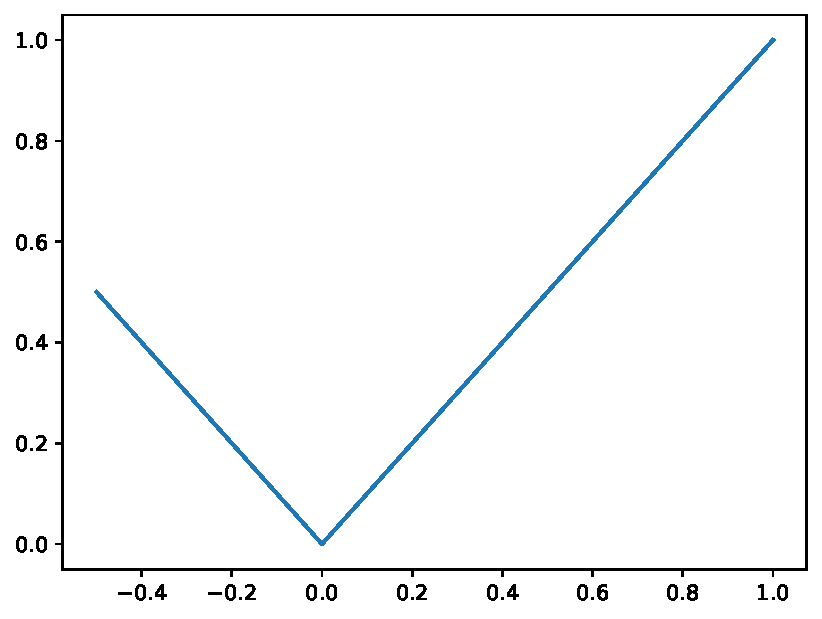
\includegraphics[width=0.8\textwidth]{./cap_ag/dados/fig_absx/fig}
    \caption{Gráfico referente ao Exemplo~\ref{cap_ag_sec_graf:ex:absx}.}
    \label{cap_ag_sec_graf:fig:absx}
  \end{figure}
  
\begin{lstlisting}
import matplotlib.pyplot as plt

# figure
fig = plt.figure()
# axes
ax = fig.add_subplot()
# plot
ax.plot([-0.5, 0, 1],
        [0.5, 0, 1])
# display
plt.show()
\end{lstlisting}
\end{ex}

No caso de curvas, podemos usamos um número adequado de pontos de forma que os segmentos de linhas ficam imperceptíveis a olho nu.

\begin{ex}\label{cap_ag_sec_graf:ex:fun}
  Consideramos a função
  \begin{equation}
    f(x) = \left\{
      \begin{array}{ll}
        -(x+1)^2-2 &, ~-2\leq x < -\frac{1}{2},\\
        |x| &, ~-\frac{1}{2}\leq x < 1,\\
        (x-2)^3 + 2, &, ~1\leq x < 3.
      \end{array}
    \right.
  \end{equation}
  A Figura~\ref{cap_ag_sec_graf:fig:fun}, mostra o gráfico de $f$ plotado com o código abaixo.

  \begin{figure}[H]
    \centering
    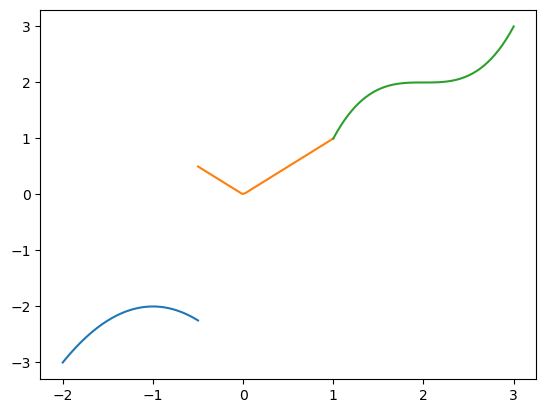
\includegraphics[width=0.8\textwidth]{./cap_ag/dados/fig_fun/fig}
    \caption{Gráfico referente ao Exemplo~\ref{cap_ag_sec_graf:ex:fun}.}
    \label{cap_ag_sec_graf:fig:fun}
  \end{figure}  

\begin{lstlisting}
import matplotlib as mpl
import matplotlib.pyplot as plt
import numpy as np

# figure
fig = plt.figure()
# axis
ax = fig.add_subplot()
# -2 <= x < -0.5
x = np.linspace(-2, -0.5)
ax.plot(x, -(x+1)**2-2)
# -0.5 <= x < 1
x = np.linspace(-0.5, 1)
ax.plot(x, np.fabs(x))
# 1 <= x < 3
x = np.linspace(1, 3)
ax.plot(x, (x-2)**3+2)
# display
plt.show()
\end{lstlisting}
\end{ex}

\subsection{Eixos}

No {\matplotlib}, os eixos de um gráfico são objetos da classe \href{https://matplotlib.org/stable/api/axis_api.html#matplotlib.axis.Axis}{\lstinline+Axis+}\footnote{Não confundir com Axes, um objeto que contém todos os elementos de um gráfico.}.

\begin{ex}\label{cap_ag_sec_graf:ex:axis}
  Com o código abaixo, produzimos a Figura~\ref{cap_ag_sec_graf:fig:eixos}, a qual contém o gráfico da função do Exemplo~\ref{cap_ag_sec_graf:fig:fun} com os eixos editados.

  \begin{figure}[H]
    \centering
    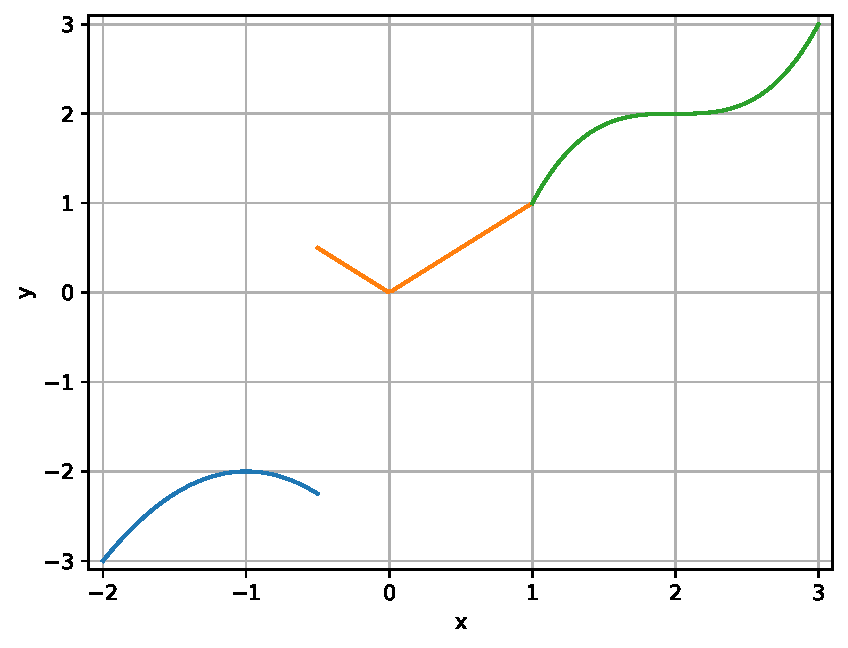
\includegraphics[width=0.8\textwidth]{./cap_ag/dados/fig_eixos/fig}
    \caption{Gráfico referente ao Exemplo~\ref{cap_ag_sec_graf:ex:eixos}.}
    \label{cap_ag_sec_graf:fig:eixos}
  \end{figure}  

\begin{lstlisting}
import matplotlib as mpl
import matplotlib.pyplot as plt
import numpy as np

# figure
fig = plt.figure()
# axis
ax = fig.add_subplot()
# -2 <= x < -0.5
x = np.linspace(-2, -0.5)
ax.plot(x, -(x+1)**2-2)
# -0.5 <= x < 1
x = np.linspace(-0.5, 1)
ax.plot(x, np.fabs(x))
# 1 <= x < 3
x = np.linspace(1, 3)
ax.plot(x, (x-2)**3+2)
# eixo-x
ax.set_xlim((-2.1, 3.1))
ax.set_xticks([-2, -1, 0, 1, 2, 3])
ax.set_xlabel('x')
#eixo-y
ax.set_ylim((-3.1, 3.1))
ax.set_yticks([-3, -2, -1, 0, 1, 2, 3])
ax.set_ylabel('y')
# grid
ax.grid()
# display
plt.savefig('fig.png', bbox_inches='tight')
plt.savefig('fig.pdf', bbox_inches='tight')
plt.show()
\end{lstlisting}
\end{ex}

\subsection{Elementos Gráficos}

No {\matplotlib}, os elementos gráficos (basicamente tudo o que é visível, pontos, linhas, eixos, etc.) são objetos da classe \href{https://matplotlib.org/stable/api/artist_api.html#artist-class}{Artist}.

\begin{ex}\label{cap_ag_sec_graf:ex:elgraf}
  Com o código abaixo, produzimos a Figura~\ref{cap_ag_sec_graf:fig:elgraf}, a qual contém o gráfico da função do Exemplo~\ref{cap_ag_sec_graf:fig:elgraf} com os eixos editados.

  \begin{figure}[H]
    \centering
    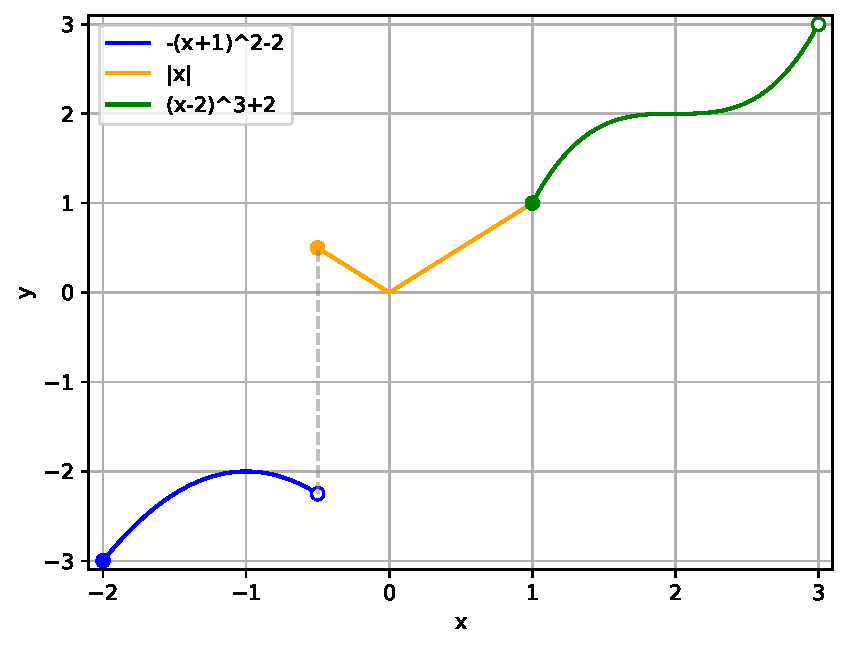
\includegraphics[width=0.8\textwidth]{./cap_ag/dados/fig_elgraf/fig}
    \caption{Gráfico referente ao Exemplo~\ref{cap_ag_sec_graf:ex:elgraf}.}
    \label{cap_ag_sec_graf:fig:elgraf}
  \end{figure}
  
\begin{lstlisting}
import matplotlib as mpl
import matplotlib.pyplot as plt
import numpy as np

# figure
fig = plt.figure()
# axis
ax = fig.add_subplot()

# -2 <= x < -0.5
x = np.linspace(-2, -0.5)
f1 = lambda x: -(x+1)**2-2
ax.plot(x, f1(x), color='blue',
        label='-(x+1)^2-2')
ax.plot([-2.], f1(-2.), linestyle='', marker='o',
        color='blue')
ax.plot([-0.5], f1(-0.5), ls='', marker='o',
        markerfacecolor='white', markeredgecolor='blue')

# -0.5 <= x < 1
x = np.linspace(-0.5, 1)
f2 = lambda x: np.fabs(x)
ax.plot(x, f2(x), color='orange', label='|x|')
ax.plot([-0.5], [f2(-0.5)], ls='', marker='o',
        color='orange')

ax.plot([-0.5, -0.5], [f1(-0.5), f2(-0.5)],
        ls = '--', color='gray', alpha=0.5)

# 1 <= x < 3
x = np.linspace(1, 3)
f3 = lambda x: (x-2)**3+2
ax.plot(x, f3(x), color='green',
        label='(x-2)^3+2')
ax.plot([1.], [f3(1.)], ls='', marker='o',
        color='green')
ax.plot([3.], [f3(3.)], ls='', marker='o',
        mfc='white', mec='green')

# eixo-x
ax.set_xlim((-2.1, 3.1))
ax.set_xticks([-2, -1, 0, 1, 2, 3])
ax.set_xlabel('x')
# eixo-y
ax.set_ylim((-3.1, 3.1))
ax.set_yticks([-3, -2, -1, 0, 1, 2, 3])
ax.set_ylabel('y')
# grid
ax.grid()
ax.legend()
# display
plt.savefig('fig.png', bbox_inches='tight')
plt.savefig('fig.pdf', bbox_inches='tight')
plt.show()
\end{lstlisting}
\end{ex}

\subsection{Textos e Anotações}

Elementos texto podem ser adicionados a um \lstinline+Axes+ com o comando \href{https://matplotlib.org/stable/api/_as_gen/matplotlib.axes.Axes.text.html#matplotlib.axes.Axes.text}{\lstinline+axes.text()+}. Anotações, consistem em um apontamento, e podem ser adicionadas com o comando \href{https://matplotlib.org/stable/api/_as_gen/matplotlib.axes.Axes.annotate.html#matplotlib.axes.Axes.annotate}{\lstinline+axes.annotate()+}. Elementos texto suportam \LaTeX usando-se o marcador de texto \lstinline!$!.%$

\begin{ex}\label{cap_ag_sec_graf:ex:texto}
  Com o código abaixo, produzimos a Figura~\ref{cap_ag_sec_graf:fig:texto}, a qual contém o gráfico da função do Exemplo~\ref{cap_ag_sec_graf:fig:texto} com os eixos editados.

  \begin{figure}[H]
    \centering
    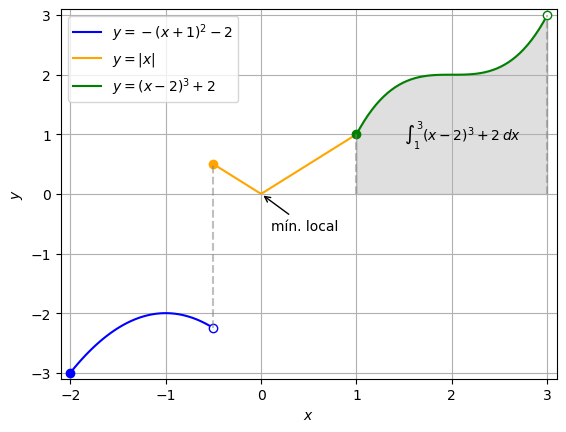
\includegraphics[width=0.8\textwidth]{./cap_ag/dados/fig_texto/fig}
    \caption{Gráfico referente ao Exemplo~\ref{cap_ag_sec_graf:ex:texto}.}
    \label{cap_ag_sec_graf:fig:texto}
  \end{figure}
  
\begin{lstlisting}
import matplotlib as mpl
import matplotlib.pyplot as plt
import numpy as np

# figure
fig = plt.figure()
# axis
ax = fig.add_subplot()

# -2 <= x < -0.5
x = np.linspace(-2, -0.5)
f1 = lambda x: -(x+1)**2-2
ax.plot(x, f1(x), color='blue',
        label='$y=-(x+1)^2-2$')
ax.plot([-2.], f1(-2.), linestyle='', marker='o',
        color='blue')
ax.plot([-0.5], f1(-0.5), ls='', marker='o',
        markerfacecolor='white', markeredgecolor='blue')

# -0.5 <= x < 1
x = np.linspace(-0.5, 1)
f2 = lambda x: np.fabs(x)
ax.plot(x, f2(x), color='orange', label='$y=|x|$')
ax.plot([-0.5], [f2(-0.5)], ls='', marker='o',
        color='orange')

ax.plot([-0.5, -0.5], [f1(-0.5), f2(-0.5)],
        ls = '--', color='gray', alpha=0.5)
# anotação
ax.annotate('mín. local', xy=(0,0), xytext=(0.1,-0.6),
            arrowprops={'arrowstyle':'->'})

# 1 <= x < 3
x = np.linspace(1, 3)
f3 = lambda x: (x-2)**3+2
ax.plot(x, f3(x), color='green',
        label='$y=(x-2)^3+2$')
ax.plot([1.], [f3(1.)], ls='', marker='o',
        color='green')
ax.plot([3.], [f3(3.)], ls='', marker='o',
        mfc='white', mec='green')

# hachurando
ax.fill_between(x, f3(x), color='gray', alpha=0.25)
ax.plot([1., 1.], [0., f3(1.)],
        ls='--', color='gray', alpha=0.5)
ax.plot([3., 3.], [0., f3(3.)],
        ls='--', color='gray', alpha=0.5)
# texto
ax.text(1.5, 0.9, '$\\int_{1}^3 (x-2)^3+2\,dx$')

# eixo-x
ax.set_xlim((-2.1, 3.1))
ax.set_xticks([-2, -1, 0, 1, 2, 3])
ax.set_xlabel('$x$')
# eixo-y
ax.set_ylim((-3.1, 3.1))
ax.set_yticks([-3, -2, -1, 0, 1, 2, 3])
ax.set_ylabel('$y$')
# grid
ax.grid()
ax.legend()
# display
plt.savefig('fig.png', bbox_inches='tight')
plt.savefig('fig.pdf', bbox_inches='tight')
plt.show()
\end{lstlisting}
\end{ex}

\subsection{Exercícios}

\begin{exer}
  Use o {\matplotlib} para produzir um gráfico para as seguintes funções:
  \begin{enumerate}[a)]
  \item $\displaystyle f(x) = x^2$, $-2 \leq x \leq 2$.
  \item $\displaystyle g(x) = 2x^3+2$, $-3 \leq x \leq 0$.
  \item $\displaystyle h(x) = \sen(x)$, $-\pi \leq x \leq \pi$.
  \end{enumerate}
\end{exer}

\begin{exer}
  Use o {\matplotlib} para plotar o gráfico da função sigmoid
  \begin{equation}
    f(x) = \frac{1}{1 + e^{-x}}.
  \end{equation}
  Na mesma área gráfica, plote retas tracejadas identificando suas assíntotas horizontais.
\end{exer}
\begin{resp}
  Dica: $y = 0$ e $y=1$ são assíntotas horizontais da função sigmoid.
\end{resp}

\begin{exer}
  Use o {\matplotlib} para plotar o gráfico de $f(x) = 1/x$, $-2 \leq x \leq 2$. Na mesma área gráfica, plote uma reta tracejada identificando a assíntota vertical de $f$.
\end{exer}
\begin{resp}
  Dica: $x = 0$ é assíntota vertical de $f$.
\end{resp}

\begin{exer}
  Use o {\matplotlib} para produzir um gráfico para a seguinte função definida por partes
  \begin{equation}
    f(x) = \left\{
      \begin{array}{ll}
        \cos(x) &, -\pi < x \leq 0,\\
        1-x^2 &, 0 < x \leq 2.
      \end{array}
    \right.
  \end{equation}
  Use de marcadores para identificar os pontos extremos de cada parte da função. Também, adicione o \textit{label} de cada eixo e uma legenda para identificar cada parte da função.
\end{exer}

\begin{exer}
  Em uma mesma área gráfica, plote as curvas $y = x + 1$ e $y = x^2$, e marque seus pontos de interseção. Para cada um destes pontos, inclua a anotação ``pto. de interseção''.
\end{exer}

\begin{exer}
  No gráfico da função sigmoid
  \begin{equation}
    f(x) = \frac{1}{1 + e^{-x}}
  \end{equation}
  hachure (pinte) a região que corresponde a área associada a integral definida
  \begin{equation}
    \int_1^3 f(x)\,dx.
  \end{equation}
\end{exer}
\begin{resp}
  Dica: use a função \href{https://matplotlib.org/stable/api/_as_gen/matplotlib.axes.Axes.fill_between.html#matplotlib.axes.Axes.fill_between}{\lstinline+Axes.fill_between()+}.
\end{resp}

\begin{ex}
  Em uma mesma área gráfica, plote a área entre as curvas $y = x + 1$ e $y = x^2$, $x=-1$ e $x=2$.
\end{ex}

\ifisbook
\subsubsection{Respostas}
\shipoutAnswer
\fi

